\documentclass[12pt, a4paper]{article}
\usepackage{indentfirst}
      \setlength{\parindent}{2em}
\usepackage{times}
\usepackage{mathptmx}
\usepackage{amsmath}
\usepackage{graphicx}
\usepackage{setspace}
    \doublespacing
\usepackage{floatrow}
\usepackage{tikz}
    \usetikzlibrary{calc, shapes, backgrounds}
\usepackage{amssymb}
\usepackage[boxed, linesnumbered, lined]{algorithm2e}
\usepackage{pgfplots}
    \pgfplotsset{compat=1.12}

\usepackage{listings}
\usepackage{float}
\lstset{ 
  backgroundcolor=\color{white},   % choose the background color; you must add \usepackage{color} or \usepackage{xcolor}
  basicstyle=\ttfamily,            % the size of the fonts that are used for the code
  breakatwhitespace=false,         % sets if automatic breaks should only happen at whitespace
  breaklines=true,                 % sets automatic line breaking
  captionpos=b,                    % sets the caption-position to bottom
  commentstyle=\ttfamily\color{blue},    
                                   % comment style
  deletekeywords={},               % if you want to delete keywords from the given language
  escapeinside={},                 % if you want to add LaTeX within your code
  extendedchars=true,              % lets you use non-ASCII characters; for 8-bits encodings only, does not work with UTF-8
  frame=single,                    % adds a frame around the code
  keepspaces=true,                 % keeps spaces in text, useful for keeping indentation of code (possibly needs columns=flexible)
  keywordstyle=\color{blue},       % keyword style
  language=Python,                    % the language of the code
  morekeywords={},                 % if you want to add more keywords to the set
  numbers=left,                    % where to put the line-numbers; possible values are (none, left, right)
  numbersep=5pt,                   % how far the line-numbers are from the code
  numberstyle=\tiny\color{black}, % the style that is used for the line-numbers
  rulecolor=\color{black},         % if not set, the frame-color may be changed on line-breaks within not-black text (e.g. comments (green here))
  showspaces=false,                % show spaces everywhere adding particular underscores; it overrides 'showstringspaces'
  showstringspaces=false,          % underline spaces within strings only
  showtabs=false,                  % show tabs within strings adding particular underscores
  stepnumber=1,                    % the step between two line-numbers. If it's 1, each line will be numbered
  stringstyle=\color{black},     % string literal style
  tabsize=2,                       % sets default tabsize to 2 spaces
  title=\lstname                   % show the filename of files included with \lstinputlisting; also try caption instead of title
}















\begin{document}

    \title{\bf Douban book crawler and analysis}
    \author{
        {Zhong Junyan\thanks{Student ID: 1909853GIM20007}}\\
        Faculty of Information Technology , M.U.S.T\\
        %
    }
    \date{}
    \maketitle

    \hrule

    \begin{abstract}
        \noindent




        {\sl With the development of the society, the demand of finding a good book \\
        is increasing.In order to find a good book,I firstly use python to crawl book details\
        from the Douban book.Secondly,I made data cleaning and then store the data into the \
        MySQL database.Thirdly I make briefly data analysis for the data.Last but not least,I add the \
        sell ratings information for my data from Amazon and then use $k$-means cluster methods to cluster \ 
        the data and then I divide my data into train set and test set and use some classification methods \ 
        to classify my data.Finally I find the Random forest classification make the best performance in \ 
        the classification of test set.}



















        {\bf Keywords:} Data crawl,Data storage,MySQL database ,$K$-means cluster, \\ Random forest classification
    \end{abstract}

    \hrule

    
    \section{Introduction}
            
        If we want to find a good book we usually refer to the 
        Douban book website.And if we want to know the popularity 
        of a book we would refer to the rank on the Amazon.Therefore I 
        got a book list and its details on Douban book and then get the 
        rank information from the Amazon.Then I make some analysis base on 
        the data.What’s more, in order to find the book which has less 
        comments on Douban book and high rank on the Amazon I make  
        cluster analysis and classification analysis for my data.I would 
        also shows the details and the optimization of the algorithms.\\

    \section{Data Crawl and analysis}
       
    The website of the Douban book is:\small $ https://www.douban.com/doulist/1264675$.\

In order to crawl the data from the website 
we firstly analyze the structure of the website:


\begin{figure}[ht]
    \centering
    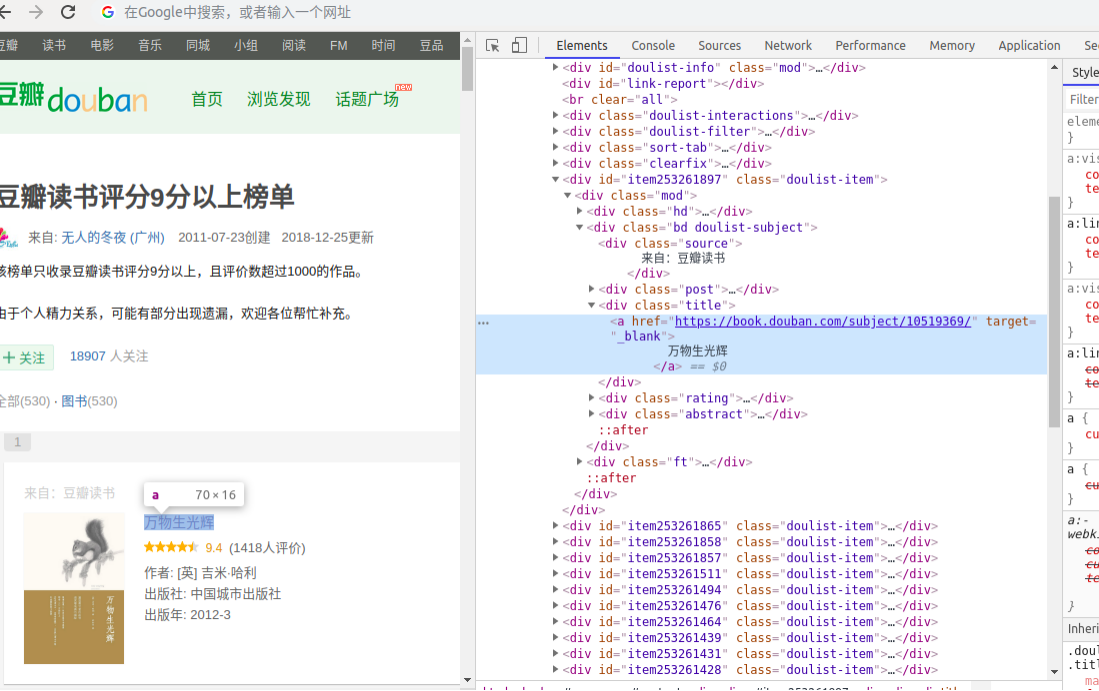
\includegraphics[width=8cm,height=7cm]{p1.png}
    \caption{Douban book website.}
\end{figure}


   \subsection{Data crawl}
   We can see that the list is controlled by the ‘’start={}’’ so we can use a 
   loop to crawl the information for the book.Then we can see that the details of 
   the book is shown in the graph above.Therefore we can use the regular expression 
   to crawl the data\cite{mitchell2018web}: 


\lstset{language=Python}
\begin{lstlisting}[caption={Data crawl}]
def getDetail(html):
     detailList=re.findall(r'<ahref="(https.*?)".*?target="_blank">.*?</a>',html,re.S)
     newDetailList = []
        for index,item in enumerate(detailList):
            if item.find("subject") != -1 and index % 2!=0:
             newDetailList.append(item);
 def getPublishYear(html):
          publishYearList = re.findall(r'<span class="pl">出版年.*?</span>(.*?)<br/>',html,re.S)
          return publishYearList
 \end{lstlisting}
                                                                                                                                                                                                  
   

\subsection{Data storage and cleaning}                                                                                                                                                                                          

After I crawl the data I use the MySQL database to store 
the data.Firstly I create a table in the database:
\newpage{}
\lstset{language=Python}
\begin{lstlisting}[caption={Creat table}]
import pymysql
conn = pymysql.connect(host = '127.0.0.1',user = 'root',passwd = '123456',db = 'sys',port = 3306,charset = 'utf8') 
cursor = conn.cursor()
sql = "create table douban9f(book_name text,score text,num text,picturelink text,publisher text,pulishyear text,ISBN text)engine innodb default charset=utf8"
try:
       cursor.execute(sql)
       conn.commit()
except:
       conn.rollback()
conn.close()

\end{lstlisting}


Then I storage the csv file into the database as follows:


\begin{figure}[ht]
    \centering
    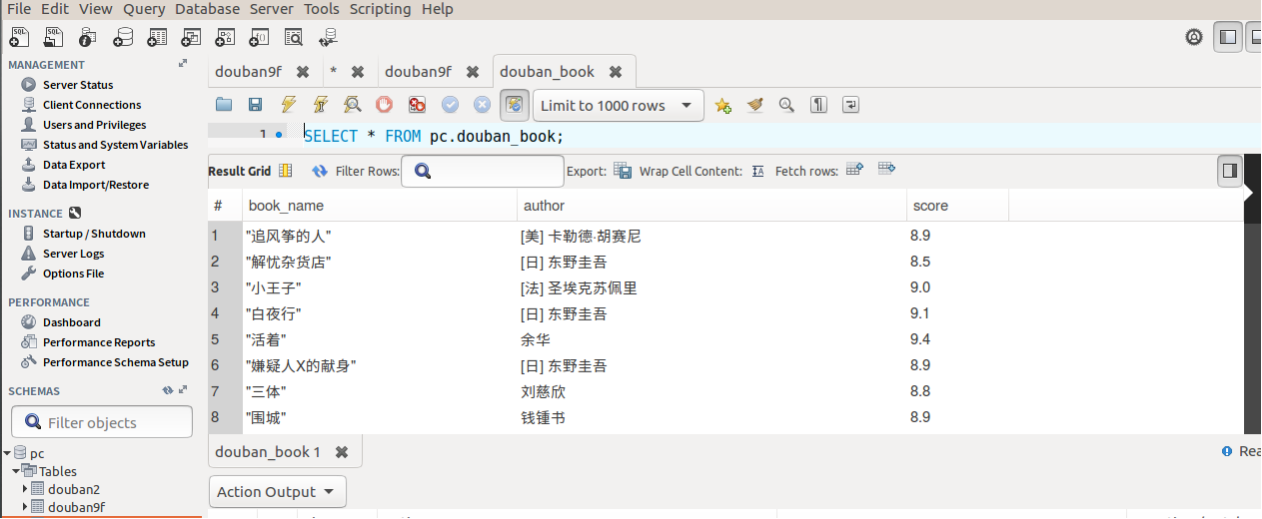
\includegraphics[width=10cm,height=5cm]{p2.png}
    \caption{Data storage.}
\end{figure}



\newpage{}
   
Then I remove the null value in my data:
\lstset{language=Python}
\begin{lstlisting}[caption={Remove the null value}]
db=pd.read_csv("9p.csv",encoding='utf-8')
db=db.dropna()
db.publishyear=pd.to_numeric(db.publishyear,downcast='integer')

\end{lstlisting}

\subsection{Data analysis}
Then we can draw the distribution of the score of 
the book as follows:

\begin{figure}[ht]
    \centering
    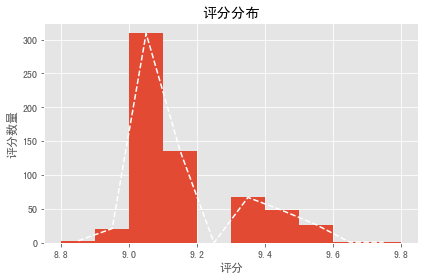
\includegraphics[width=10cm,height=4cm]{p3.png}
    \caption{Score distribution.}
\end{figure}

\begin{figure}[ht]
    \centering
    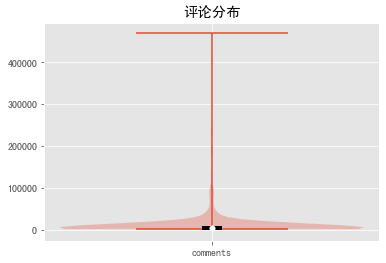
\includegraphics[width=10cm,height=5cm]{p4.png}
    \caption{Comments distribution.}
\end{figure}

\newpage{}

We can see that the score of the book densely distributed on the 
interval of 9.0 to 9.2 and we can see that many books’ comments 
is less than 10000.

Then I plot the following graph base on my data and get the 
top10 books which have the most comments and the average 
comments of each year:

\begin{figure}[ht]
    \centering
    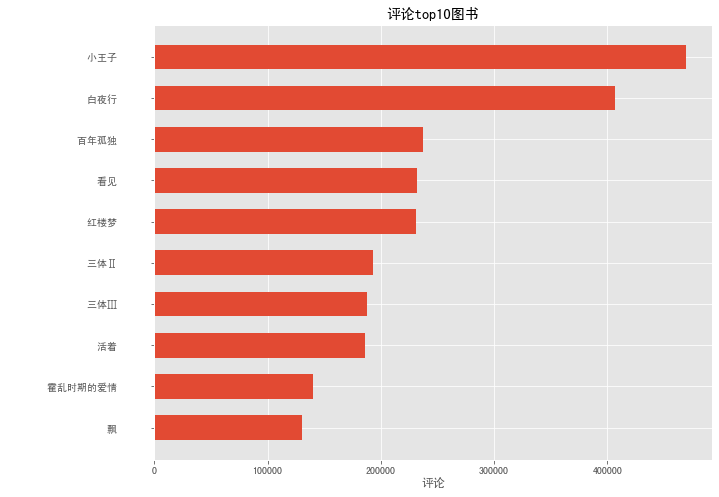
\includegraphics[width=10cm,height=6cm]{p5.png}
    \caption{Top10 comments books.}
\end{figure}

\begin{figure}[ht]
    \centering
    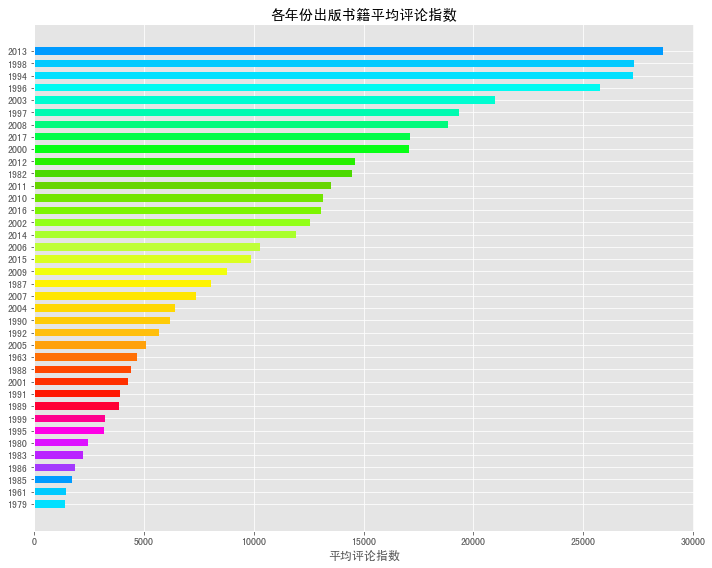
\includegraphics[width=12cm,height=6cm]{p6.png}
    \caption{Average comments of each year.}
\end{figure}

\newpage{}

\subsection{Conclusion}
We can draw a conclusion that the book with high score may not have high popularity.
Therefore,we shall create a new way to recommend books to others in a new way 
which both refer to the popularity of the book and the score of the book.



\newpage
\section{Clustering and classification}





\subsection{PCA}
PCA is a statistical process\cite{bishop2006pattern} that uses 
an orthogonal transformation to transform 
the observations set of possibly related variables 
into a set of linearly uncorrelated variables.In order to 
reduce the dimensionality of features I use the PCA
to extract the two most influential features for analysis.
\lstset{language=Python}
\begin{lstlisting}[caption={PCA}]
pca=PCA(n_components=2)
X=data[cols]
NX=pca.fit_transform(X)
NX=abs(NX)
\end{lstlisting}
In order to simplify the following work, I turn eigenvectors positive value.


\subsection{Clustering}
      $k$-means clustering\cite{wagstaff2001constrained} is a well-known phenomenon in geometric data, and has application in machine learning. 
        To simplify the problem, we define the distance function in standardized 
        euclidean metric:

        \begin{equation*}\begin{split}
            d(p,q)&=\sqrt{(q_{1}-p_{1})^2+(q_{2}-p_{2})^2+\cdots+(q_{n}-p_{n})^2}\\
            &=\sqrt{\sum_{i=1}^{n}{(q_{i}-p_{i})^2}}
        \end{split}\end{equation*}


   
   We use the knn function to select the best value of K as follows:

   \begin{figure}[ht]
    \centering
    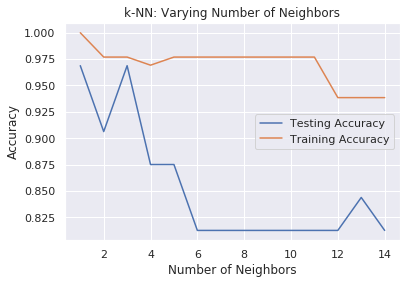
\includegraphics[width=8cm,height=5cm]{p7.png}
    \caption{Select best K value.}
\end{figure}
   \newpage
   We can that K=3 is the best value for the $k$-means clustering
   so we use K=3 to cluster the data.
   
   

   \begin{figure}[ht]
    \centering
    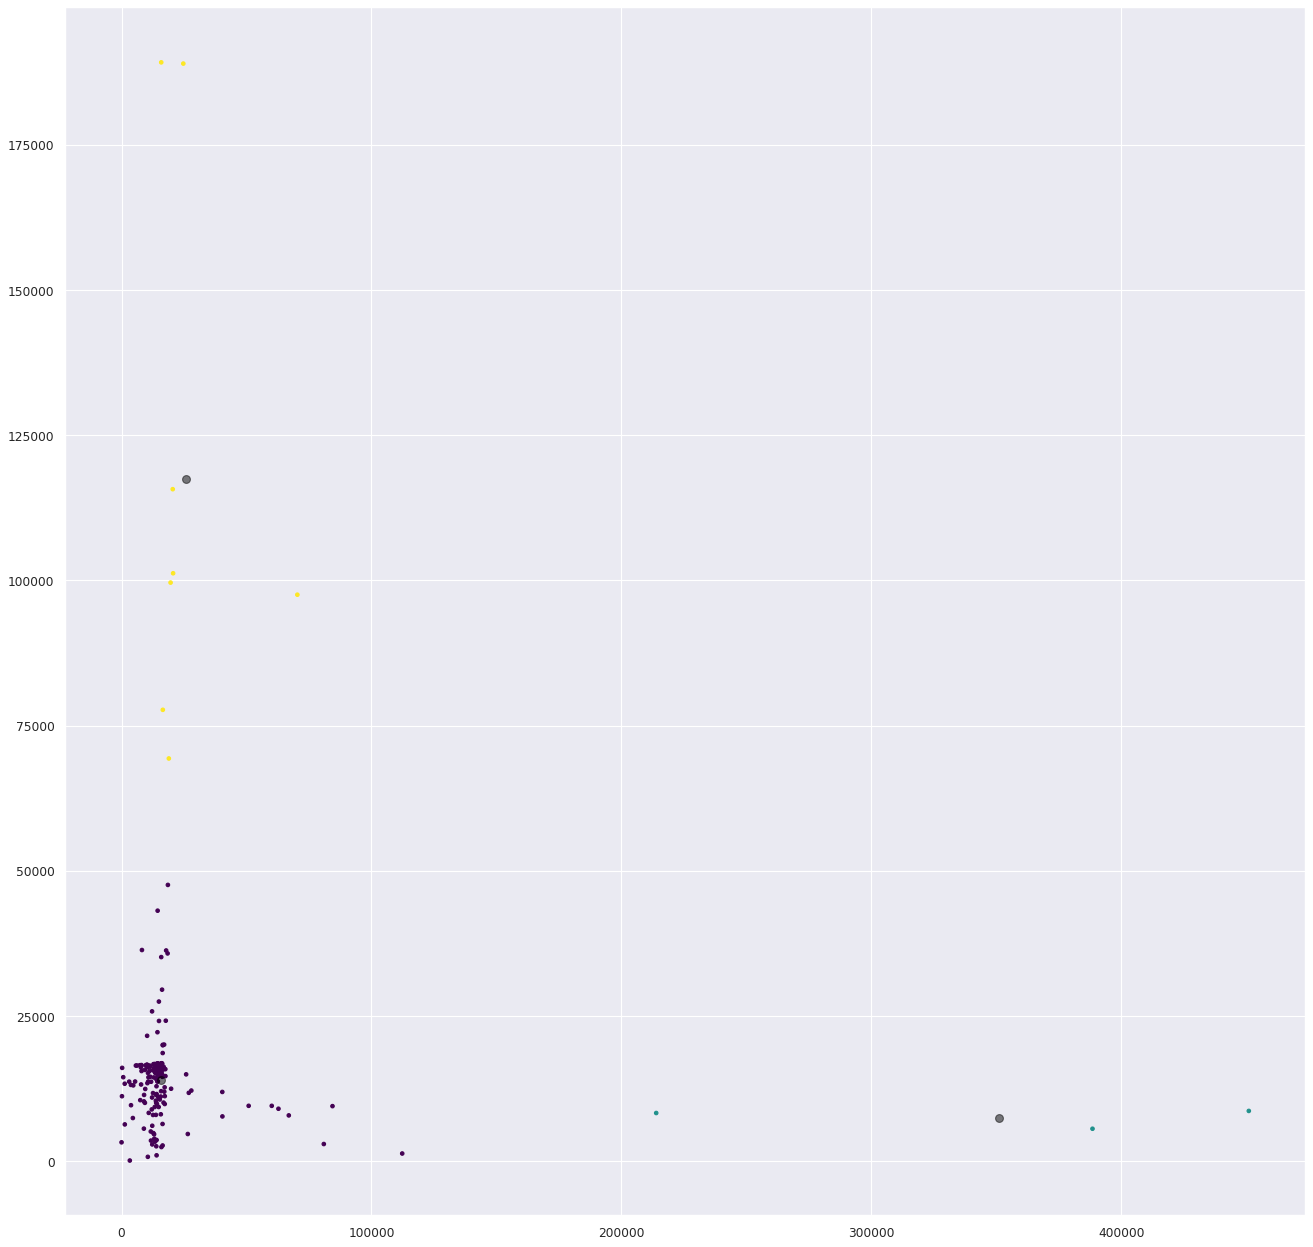
\includegraphics[width=12cm,height=8cm]{p8.png}
    \caption{Cluster plot.}
\end{figure}
\newpage
\subsection{Classification}
In order to find  find some books which are unpopular 
in douban but it's popular in amazon I select the most 
 dense clusters for analysis.Then I select the first 130
 samples as the train data set and rest of the data as 
 the test data set.Then I use four classification methods\cite{vanderplas2016python} to classify
 the data and see which classification methods make the best performance
 in the test data set.

   \subsubsection{Linear-SVM classification method}
Firstly I use Linear-SVM classification method\cite{chang2008feature} to classify the data. 
\begin{figure}[ht]
    \centering
    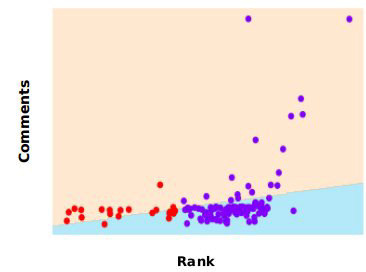
\includegraphics[width=10cm,height=6cm]{p9.png}
    \caption{LSVM classification.}
\end{figure}
\newpage
\subsection{logistic regression classification method}
The second method I used is the logistic regression classification.

\begin{figure}[ht]
    \centering
    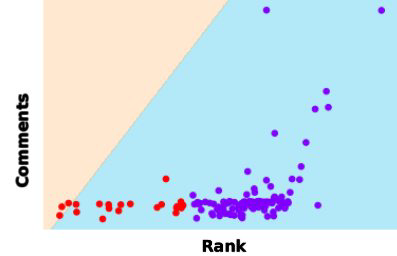
\includegraphics[width=10cm,height=6cm]{p10.png}
    \caption{Logistic regression classification.}
\end{figure}

\subsection{Decision tree classification method}
The third method I used is the Decision tree method.And we can see that the effect
of this method has significant improved than the above two methods.

\begin{figure}[ht]
    \centering
    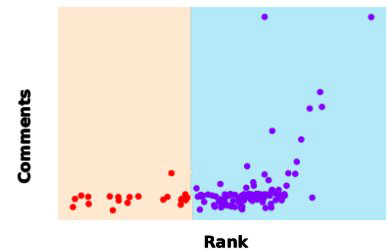
\includegraphics[width=10cm,height=6cm]{p11.png}
    \caption{Decision tree classification train set.}
\end{figure}
    \begin{figure}[ht]
        \centering
        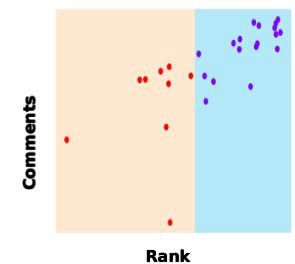
\includegraphics[width=10cm,height=6cm]{p12.png}
        \caption{Decision tree classification test set.}
 \end{figure}

\newpage
\subsection{Random forest classification method}
 The last method I used is the Random forest classification method\cite{liaw2002classification}.
 This algorithm is an improved algorithm based on the decision tree 
 classification algorithm.
 It aggregates the votes from different decision trees 
 to decide the final class of the test object.



 \begin{figure}[ht]
    \centering
    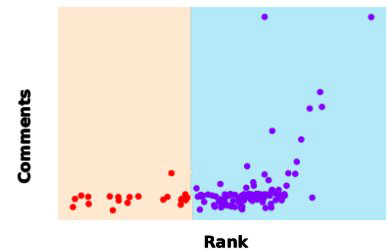
\includegraphics[width=10cm,height=6cm]{p13.png}
    \caption{Random forest classification train set.}
\end{figure}

\begin{figure}[ht]
    \centering
    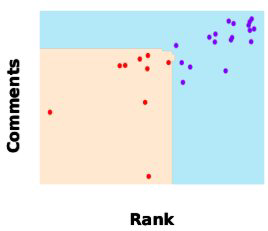
\includegraphics[width=9cm,height=5cm]{p14.png}
    \caption{Random forest classification test set.}
\end{figure}
\pagebreak[4]
Then we can see the Random forest as follows:

\begin{figure}[ht]
    \centering
    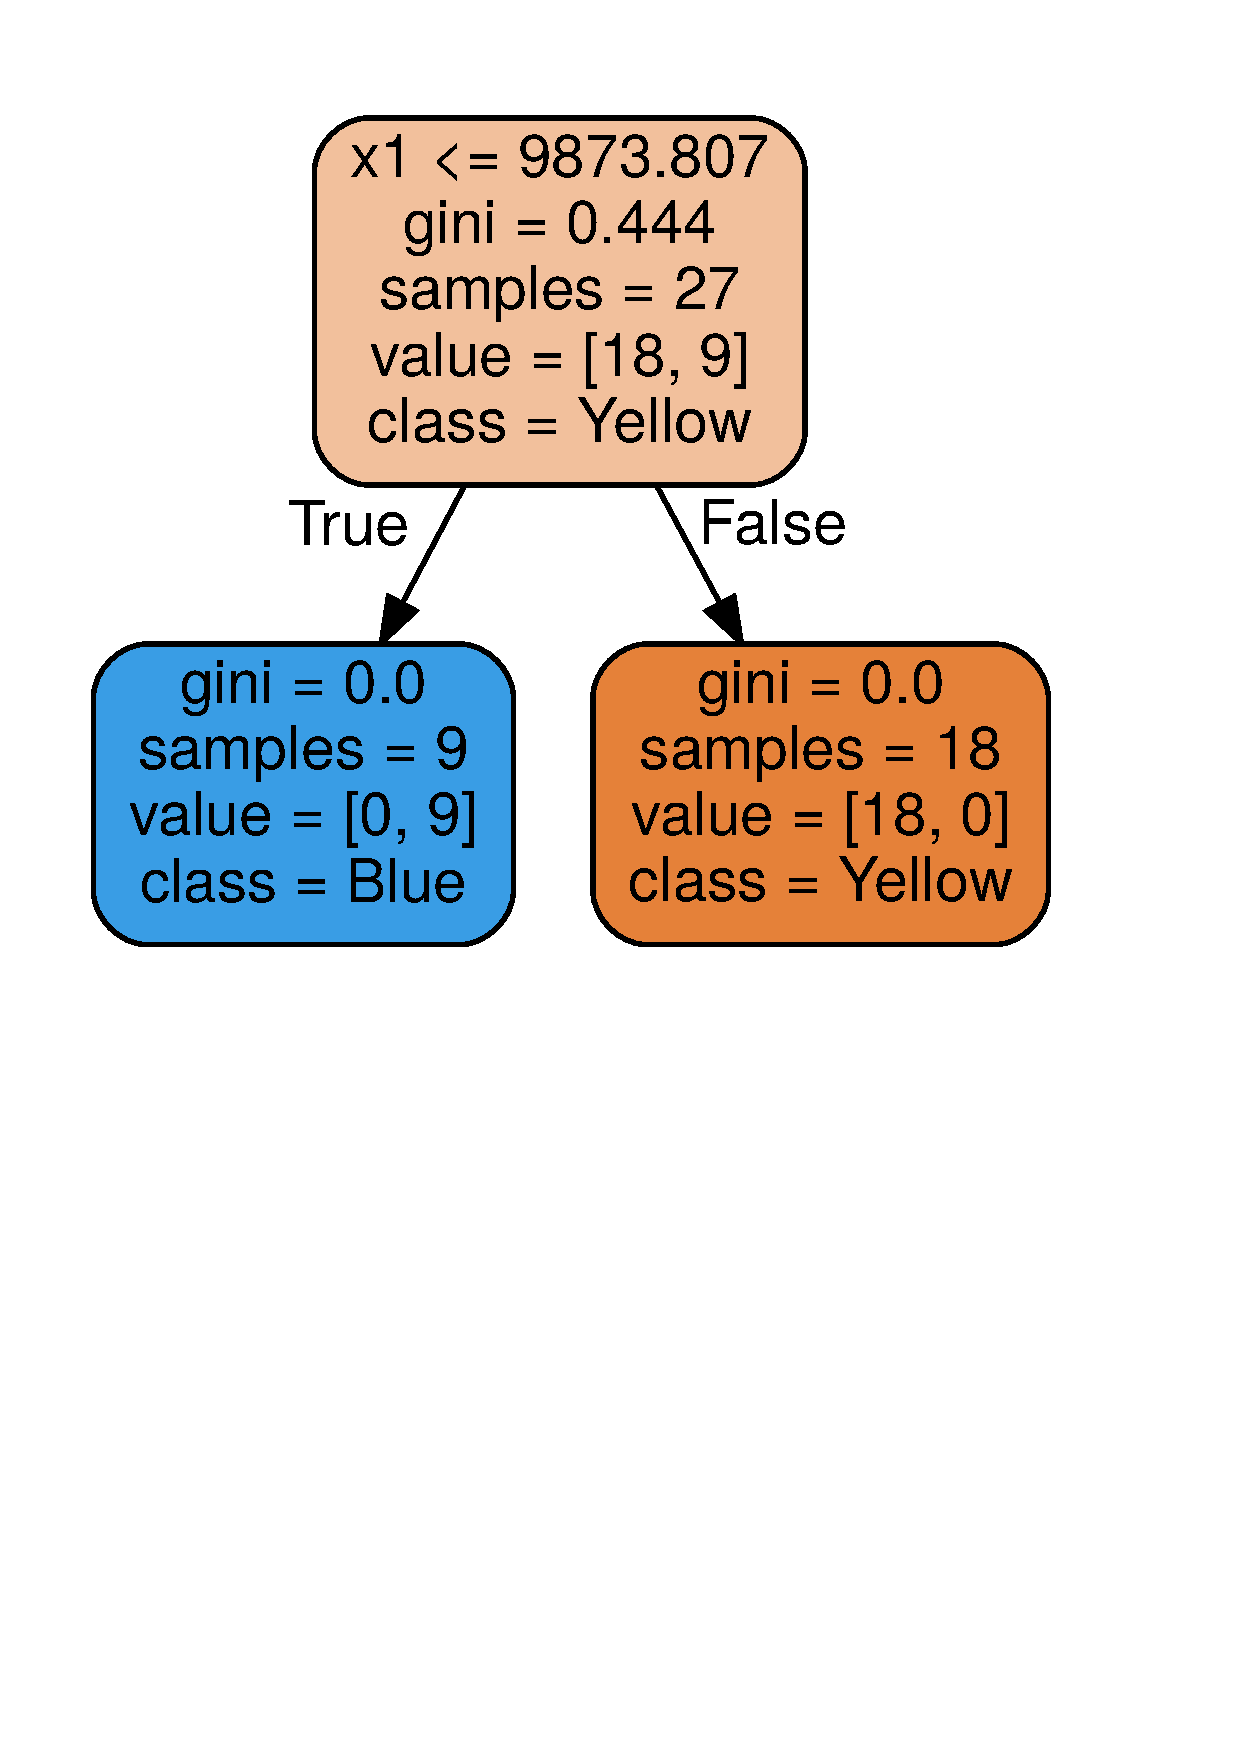
\includegraphics[width=6cm,height=8cm]{p15.pdf}
    \caption{Random forest.}
\end{figure}
\newpage
\subsection{Conclusion}
We can draw a conclusion that the random forest classification make
the  greatest \\performance in the classification test.
And the score for each method performance are \\as follows:
\newline

  
    
    \begin{table}[H]
    \begin{tabular}{|l|l|}

    \hline
    methods             & score \\ \hline
    Lsvm                & 0.875 \\ \hline
    Logistic regression & 0.75  \\ \hline
    Decision tree       & 0.875 \\ \hline
    Random forest       & 1     \\ \hline
 
    \end{tabular}
    \caption{Classification methods comparsion} \label{tab:sometab}
\end{table}

\newpage   
\section{Discusion}
Our web crawler can be imporved in the following way:

1.Firstly,we should set a reasonal  sleep function which can aviod the block of the website. 

2.Secondly,we can turn our Single thread web 
crawler to multi thread web crawler,\\which can 
improve the speed of our web crawler.

3.Lastly,we may try using distribution web crawler(like redis) when
we crawl Large amounts of data .

And in the $k$-means clustering we can use the k-d tree methods to 
improve the speed of the algorithm.

\section{Conclusion}
My project is including data crawling and data storage as well as data 
analysis.Then I do use clustering and classification for my data.Although 
the work is hard I try my best to finishing the work.And I learn 
a lot in this project and I would keep making progress in coding
and learning other tools in reasearch. 









\newpage



\bibliographystyle{unsrt}
\bibliography{junyanzhong}

\end{document}
